Subdivision algorithms contain two major components: \emph{topology
refinement} and \emph{geometry smoothing}.  The topology refinement
reparameterizes the source mesh into the target mesh. The geometry
smoothing maps a \emph{stencil} on the source mesh to a vertex on the
target. Any proper combination of a refinement and a set of stencil
rules defines a subdivision scheme.

Based on the \emph{policy-based design} \cite{a-rotm-02}, the
combination can be designed as a refinement function (\emph{host
function}) parameterized with the stencil rules (\emph{policy
functions}). For example, a Catmull-Clark subdivision can be
represented as a primal quadralization function with the Catmull-Clark
stencil rules.
\begin{lstlisting}
void CatmullClark_subdivision(Polyhedron& p) {
  quadralize_polyhedron<CatmullClark_rule<Polyhedron>>(p);
}
\end{lstlisting}
These policy functions modify the target vertex based on the stencil
of the source mesh. The policy set are defined according to the host
fuction, i.e.\ the refinement scheme. For primal quadralization, the
set includes functions for facet, edge and vertex stencils. In the C++
format, the policy class of the Catmull-Clark subdivision is like,
\begin{lstlisting}
class CatmullClark_rule {
public:
  void facet_rule(Facet_handle facet, Point& pt);
  void edge_rule(Halfedge_handle edge, Point& pt);
  void vertex_rule(Vertex_handle vertex, Point& pt);
};
\end{lstlisting}

To define a subdivision, we implement the refinement and the
subdivison rules separately.  The subdiviison rules is a simplified
mesh traversal problem as only the attributes of the stencil (usually
a 1-ring) need to be visited and collected. To implement a facet
stencil of the Catmull-Clark subdivision, we collect the vertices of
the facet and apply the stencil weight.
\begin{lstlisting}
void facet_rule(Facet_handle facet, Point& pt) {
  Halfedge_around_facet_circulator hcir = facet->facet_begin();
  Vector vec = hcir->vertex()->point() - CGAL::ORIGIN;
  ++hcir;
  do {
    vec = vec + hcir->vertex()->point();
  } while (++hcir != facet->facet_begin());
  pt = CGAL::ORIGIN + vec/circulator_size(hcir);
}
\end{lstlisting}

The points generated from the policy functions are stored in a
temporal geometry buffer. The order of the storage coincides to the
primitive creation of the topology refinement.

Implementating a topology refinement is a rather complex job.  One
approach is to encode the refinement into a sequence of Euler
operations. For Catmull-Clark subdivision, the refinement is encoded
as edge-vertex insertions, edge insertion between two neighboring
edge-vertices, facet-vertex insertion on he inerted edge, and then
edge insertions between the facet-vertex the edge-vertices. The
sequence of the vertex insertions matches the fetching order of the
temporal geometry buffer of the smoothed points. The sequence is
demonstrated in Figure \ref{fig:CCRefinement}. Note that the vertex
and edge insertions can be easily implemented based on the Euler
operations supported by \cgalpoly.

\begin{figure}
  \centering
  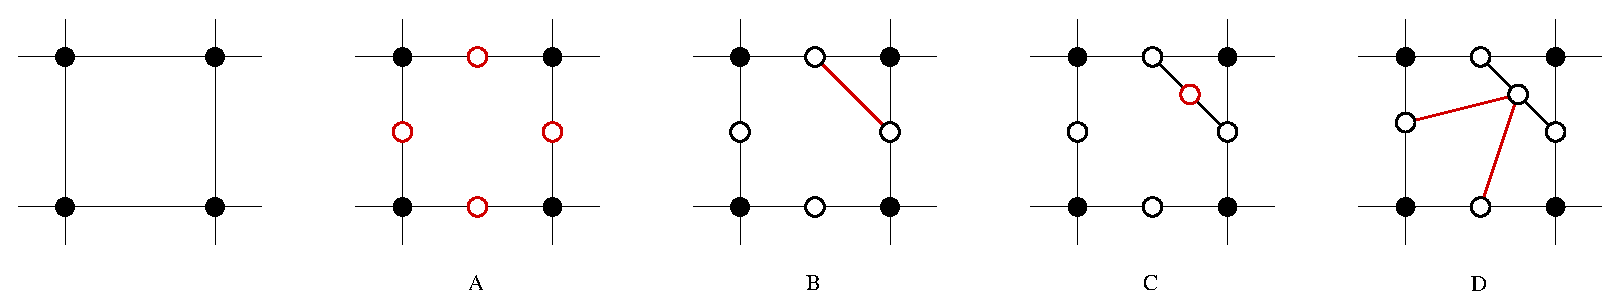
\epsfig{file=figs/CCRefinement.eps, width=7cm}
  \caption{A PQQ refinement of a facet is encoded into a sequence of
  vertex insertions and edge insertions. Red indicates the inserted
  vertices and edges on each step.}
  \label{fig:CCRefinement}
\end{figure}

Most primal refinement schemes can be translated into a sequence of
Euler operations. Though dual schemes, e.g.\ Doo-Sabin subdivision,
have no simple translation of Euler operations.  To support such
schemes, we use the modifier callback mechanism of \cgalpoly\ to
rebuild the mesh connectivity. In addition to the points buffer, we
also create a facet list based on the source mesh. Note that in DQQ
scheme, every new facet corresponds to a vertex, edge or facet. The
combination of the points buffer and facet list represents a
facet-vertex index list which indexes the vertices and enumerate each
facet as an index sequence. A modifier creating a polyhedron from a
facet-vertex index list is then a simple task.

\begin{lstlisting}
  pb.begin_surface(num_point, num_facet); {
    for (int i = 0; i < num_point; ++i) 
      pb.add_vertex(Point(point_buffer[i*3+0], 
			  point_buffer[i*3+1], 
			  point_buffer[i*3+2]));	
    for (int i = 0; i < num_facet; ++i) {
      pb.begin_facet(); {
	for (int n = 0; n < facet_buffer[i][0]; ++n)
	  pb.add_vertex_to_facet(facet_buffer[i][n+1]);
      }
      pb.end_facet();
    }
  }
  pb.end_surface();
\end{lstlisting}

Our subdivision solution accepts a generic polyhedron as the input.
The only requirement of the polyhedron is the point attribute of a
vertex. For a non-CGAL Point type, users only need to replace the
stencil policies.  The solution is natually fit in the multipass
paradigm.  A composite subdivision can be achieved by,
\begin{lstlisting}
void MySubdivision(Polyhedron& p) {
  quadralize_polyhedron<Myrule_1<Polyhedron>>(p);
  dualize_polyhedron<Myrule_2<Polyhedron>>(p);
} 
\end{lstlisting}


%The host function, i.e.\ the refinement, cannot use any
%flag to register the correspondence between the refinement.
%The policy functors should grant the access any attributes
%of any specialized polyhedron. The policy functors also
%need to be complete covering all cases, e.g.\ interior and
%boundary.

%TODO: since the writing memory is not overlapped, multi-threaded
%supporting is easily done.

%TODO: trade-off between generic and efficient.
 
